\documentclass[12pt]{article}
\usepackage[english]{babel}
\usepackage{amsmath,amsthm}
\usepackage{graphicx}
\usepackage{caption}
\usepackage{subcaption}
\usepackage{amsfonts}
\usepackage{indentfirst}
\usepackage{lscape}
\usepackage[top=2.5cm,bottom=2.5cm,right=2.5cm,left=2.5cm]{geometry}
\usepackage{titlesec}
\setcounter{secnumdepth}{5}

% ----------------------------------------------------------------
\begin{document}

\section{Quantification}

The Quantification is the step we will use for determine which images correspond to which species. For that we will use the bag of words in a first place to simplify the signature of whole images. And after use the K-nn method for the classification.

\subsection{Bag of words}

In the bag of words method we found two different step, the calculation of K-means and the design of a signature for the images.

\subsubsection{K-means}

The K-means is a simply method which consist to reduce the number of points or vectors in our case. The first step is to determinate randomly k centroid vectors, after with an Euclidean distance \eqref{euclid} we attribute the descriptors to whole images to the nearest centroid vectors.

\begin{equation}
\sum_{k=0}^{centroid}\sum_{i=0}^{desc}\parallel x_k - u_i \parallel ^2
\label{euclid}
\end{equation}

The last stage is an update step, for each centroid vectors we calculate the means of whole the descriptors associate to, so we obtain a new centroid vectors. And we applicate this algorithm for x iteration choose by the user.

For an application on a cloud of points we obtain this kind of result:



\subsubsection{Signature}

The creation of the signature is the last step of the bag of words method, they consist to assign to each images a signature in function of the number of word in the image. The graphic representation of this signature is a histogram:

\begin{figure}[h]
        \centering
        \begin{subfigure}[b]{0.5\textwidth}
                \centering
                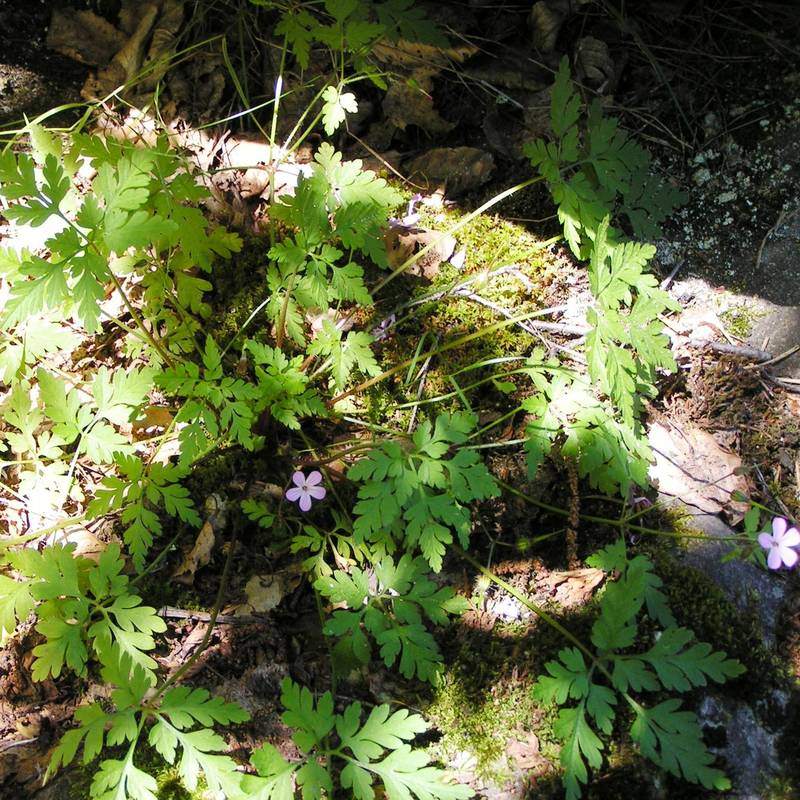
\includegraphics[height=180px]{128.jpg}
        \end{subfigure}%
        \hfill
        \begin{subfigure}[b]{0.5\textwidth}
                \centering
                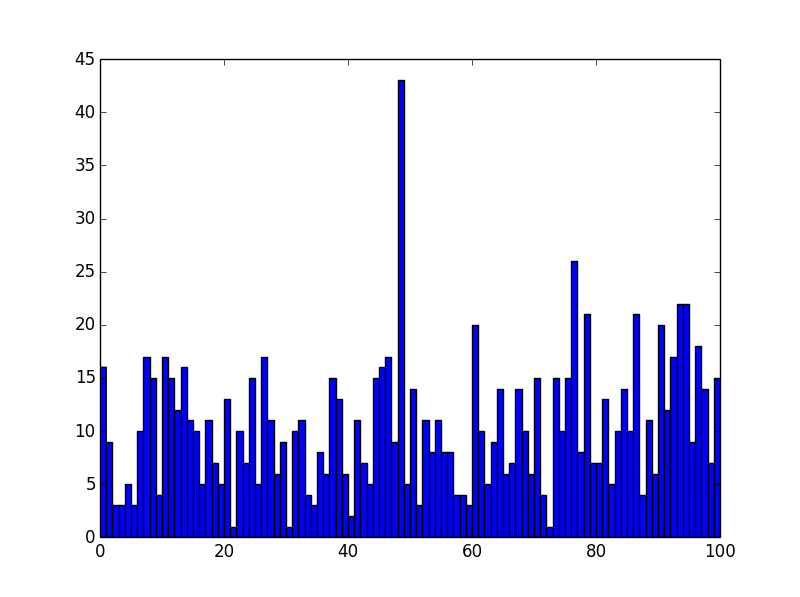
\includegraphics[height=180px]{128_sig.png}
        \end{subfigure}
        \caption{Signature de l'image 128}
        \label{fig:signature1}
\end{figure}

\begin{figure}[h]
        \centering
        \begin{subfigure}[b]{0.5\textwidth}
                \centering
                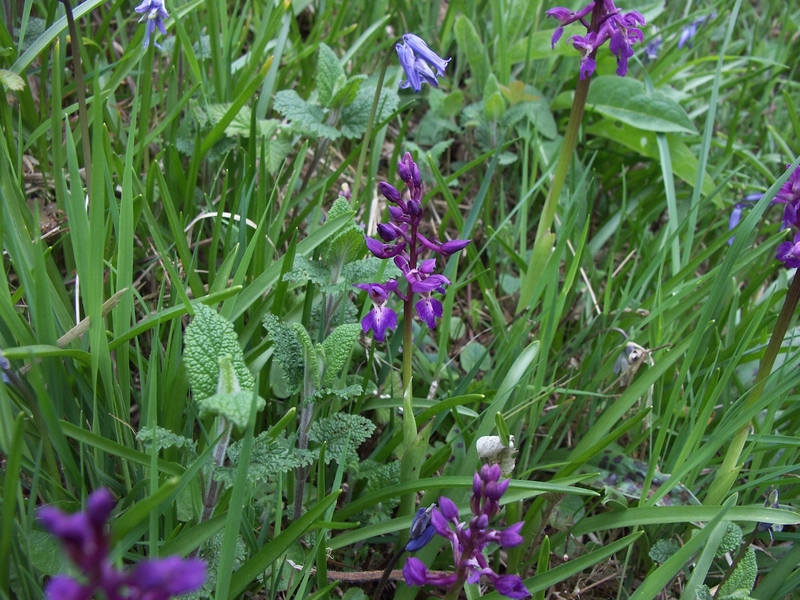
\includegraphics[height=180px]{132.jpg}
        \end{subfigure}%
        \hfill
        \begin{subfigure}[b]{0.5\textwidth}
                \centering
                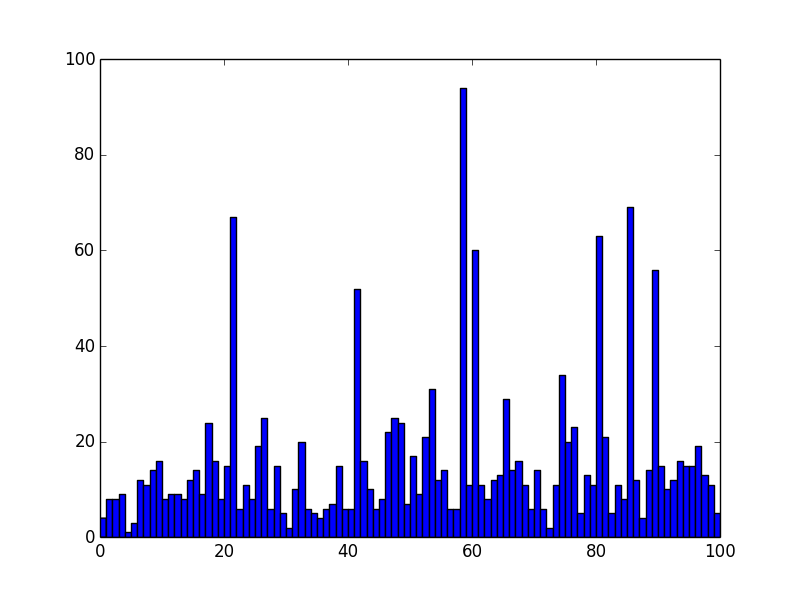
\includegraphics[height=180px]{132_sig.png}
        \end{subfigure}
        \caption{Signature de l'image 132}
        \label{fig:signature1}
\end{figure}

\subsection{K-nn}
\subsubsection{The K-nn method}
The K-nn method is one of the most simple technique in the classification field. This method consist in associating the data to classify with the class that correspond the best to it.
It is a supervised learning method : it means that the k-nn has to have a dictionary which contains all the training data sorted by class. To classify a new data, the k-nn calculates the distance between each training data and the new data. After doing that, it will simply takes the 'k' smallest ones, and determine in which class t have to attribute the new data by taking the one which is the most occurrent in the 'k' smallest distances.

For our project, the data to classify are images and the classification is made by the signature vector extracted by the K-means method. The principle is exactly the but the distances are calculated on the signature vector.
We had choose two possibilities for the distance calculation : the Euclidian distance and the $\chi^2$ distance which are described below.
\begin{itemize}
\item Euclidian distance
\vspace{0.5cm}
\begin{equation}
D_{Euc}(v_1,v_2) = \sum{(v_1(i)-v_2(i))^2}
\end{equation}

\item $\chi^2$ distance
\vspace{0.5cm}
\begin{equation}
D_{\chi^2}(v_1,v_2) =  \sum{\frac{(v_1(i)-v_2(i))^2}{(v_1(i)+v_2(i))^2}}
\end{equation}

\end{itemize}

The choice of the type of distance calculation depends on the type of descriptor chosen for the classification. For SIFT descriptor,the Euclidian distance is appropriate but each descriptor must have one distance which work better than others.
That's why the $\chi^2$ distance has been integrate in the program.

\subsubsection{Validation step}

To validate this classification method, the most simple way is to test it on artificial signatures with different constant values.
The test to validate is to take as our initial dictionary 7 vectors which we consider to be in 2 different classes. These vectors are full of constant values, they are shown as lines blow : 

\begin{figure}[h]
    \center
    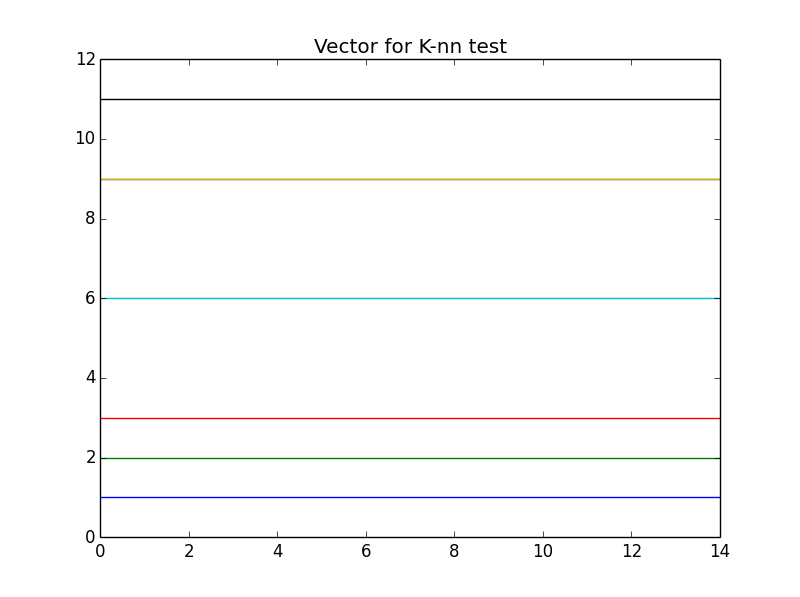
\includegraphics[scale=0.65]{knnTestVec.png}
    \caption{Dictionary of vector for k-nn tests}\label{fig:Color Difference by image shifting illustration}
\end{figure} 

The lowest one (from 0 to 3) are attributed to the first class and the others are attributed to the second one.
After that, we simply have to test to classify a signature which is constructed on the same model. When the signature vector is closer of 3 than of 6, he has to be attributed to the first class, and to the second when he is closer of 6.

The result obtained by our K-nn function is the same that the one we expected so we can say that the functioning of it is valid. 

% ----------------------------------------------------------------
\end{document} 